\section{Grammatical evolution}
\subsection{Definition}
Grammatical evolution is a evolutionary computation technique used to evolve computer programs which have a high fitness in regards to a fitness function, or in other words, which do some certain task well. The phenotypes of the individuals are executable computer programs. The genotypes of the individuals are arrays of 8-bit numbers, called codons. Authors of the algorithm have propposed using 8-bit codons in \citep{neill2003grammaticalevolution}. They've also ran some experiments with 12-bit codons and 16-bit codons, and the results have shown that increasing the codon size can result in slower evolutionary search. The genotype-phenotype mapping is done using a context-free grammar which generates the language of the desired solutions.

The process of the genotype-phenotype mapping works as follows: we start at the first codon in individual's genotpye, and we traverse the parsing tree using depth-first search, until we find a nonterminal symbol. Once we find a nonterminal symbol, we check all productions of our specified grammar in which this nonterminal symbol is the left side (head). We calculate which production to apply on this nonterminal symbol using the formula
$$Production\:=\:(Codon\:integer\:value)$$
$$MOD$$ 
$$(Number\:of\:productions\:for\:the\:current\:nonterminal\:symbol)$$ 

Once we apply the chosen production, we move on to the next codon. If we have reached the end of codon array, we move to the first codon, and this process is called wrapping. In practice, the maximum number of wrappings is specified, in order to avoid infinite recursions, and if the process exceeds this maximum number of wrappings, the mapping fails and the individual's fitness is set to the lowest possible value.

This process of traversing the parsing tree and applying grammar productions continues until there are no more nonterminal symbols in the parsing tree, and at that point the mapping is complete \citep{neill2003grammaticalevolution}.

\subsection{Properties}
Grammatical evolution has some interesting unique properties, namely the wrapping operator and code degeneracy \citep{neill2003grammaticalevolution}. 

During the genotype-phenotype mapping process, an individual could run out of codons. In that situation, the wrapping operator is applied, which means that the mapping continues from the first codon. This technique draws inspiration from a phenomen exhibited by bacteria, viruses and mitochondria which allows them to reuse the same genetic material for the expression of different genes \citep{neill2003grammaticalevolution}.

Code degeneracy refers to the fact than the mapping process used in grammatical evolution is many-to-one. Many different codon configurations in the genotype can map onto the same phenotype program. For example, during the mapping process, if the current nonterminal symbol has two different productions as specified by the grammar, then the first production would be chosen if the current codon value is even, and the second production would be chosen if the current codon value is odd. This is because $0\:MOD\:2\:=2\:MOD\:2\:=4\:MOD\:2\:=6\:MOD\:2\:=\:...\:=254\:MOD\:2\:=0$, and $1\:MOD\:2\:=3\:MOD\:2\:=5\:MOD\:2\:=7\:MOD\:2\:=\:...\:=255\:MOD\:2\:=1$. The values are shown up to 254 and 255 because these are the largest even and odd numbers, respectively, that fit into the 8 bits of one codon. This property of the genotype-phenotype mapping which enables it to have many different genotypes which all map to the same phenotpye cultivates the genetic diversity of the population \citep{neill2003grammaticalevolution}.

Grammatical evolution has some drawbacks, namely low locality and high redundancy. Low locality refers to the property of the genotype-phenotype mapping that small changes in genotype can cause drastic changes in phenotype, or even completely different phenotypes. High redundancy refers to the fact that the genotype-phenotype mapping is many-to-one, which means that many different genotypes can map to a single phenotype. Because of these two properties, the evolutionary search process in grammatical evolution can sometimes behave like random search \citep{megane2022coevolutionary}. To solve these problems, some extensions of the standard grammatical evolution have been proposed, like the structured grammatical evolution \citep{lourenco2018structured}.

\subsection{Demonstration of the genotype-phenotype mapping process}
To demonstrate the process of the genotype-phenotype mapping in the grammatical evolution, we will define a context-free grammar and one individual's genotype, and then show a step by step mapping from the genotype to the phenotype. Instead of defining a grammar using the $(V, T, P, S)$ 4-tuple, we will define it using the BNF notation. Terminal symbols are written as lowercase symbols, nonterminal symbols are written as uppercase symbols surrounded by the symbols '<' and '>', and the first nonterminal symbol is the start symbol. Production heads are written on the left side of the '::=' string, and on the right side of this string are bodies of productions which share their left side, separated by the symbol '|'. We will define our grammar as:

\noindent
$ {<}S{>}\:::=\:a\:{<}A{>}\:b\:{<}S{>}\:|\:{<}C{>}\:d\:{<}A{>}\:$\\
$ {<}A{>}\:::=\:c\:{<}B{>}\:{<}A{>}\:c\:|\:a\:b\:{<}C{>}\:|\:d $\\
$ {<}B{>}\:::=\:{<}S{>}\:a\:{<}S{>}\:|\:{<}C{>}\:d\:{<}A{>}\:|\:b\:d $\\
$ {<}C{>}\:::=\:c\:{<}C{>}\:|\:{<}C{>}\:d\:{<}C{>}\:|\:a $\\

We will also define one individual with the genotype: 
$$ [\:176,\:49,\:168,\:253,\:8,\:65,\:127,\:26,\:130,\:100\:] $$

All the intermediate strings will be displayed like linear strings, which can be constructed by traversing the parsing tree in depth.

Each step of the mapping process will be followed by a figure showing the current state of the process visually. On the top of all figures is the unit's genotype shown as a array. All the fields in this array are colored ih blue, except for the one which the index used in mapping at this turn points to, as this field is colored in yellow. Beneath the genotype array will be the parsing tree built up to that point. The nonterminal symbol which will be expanded at this turn is colored in red. The nonterminal symbols which have already been expanded are colored in green, and the nonterminal symbols which haven't yet been expanded and won't be at this turn, but sometime later in the future are colored in orange. Finally, the leaves of the tree, which are the terminal symbols, are colored in brown. These figures were built using the tool \citep{diagrams}.

The mapping process starts with the string ${<}S{>}$, and the index $i = 0$ in the genotype array. Since $i = 0$, the codon value we will use at this step is $176$. The first nonterminal symbol in the string is ${<}S{>}$, and it has $2$ productions defined in the grammar. So we calculate $176\:\:MOD\:\:2\:=\:0$, and apply the production at index $0$, which is ${<}S{>}\:::=\:a\:{<}A{>}\:b\:{<}S{>}$.

\begin{figure}[H]
	\centering
	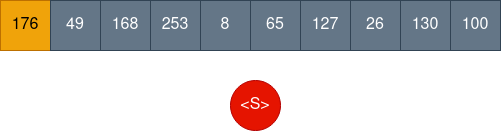
\includegraphics[scale=0.6]{parsing_tree_01.png}
	\caption{Genotype-phenotype mapping, step 1}
\end{figure}

Our current string is $a\:{<}A{>}\:b\:{<}S{>}$, the index value is $i = 1$, and the codon value is $49$. The leftmost nonterminal symbol is ${<}A{>}$, which has $3$ productions defined. So we calculate $49\:\:MOD\:\:3\:=\:1$, and apply the production at index $1$, which is ${<}A{>}\:::=\:a\:b\:{<}C{>}$

\begin{figure}[H]
	\centering
	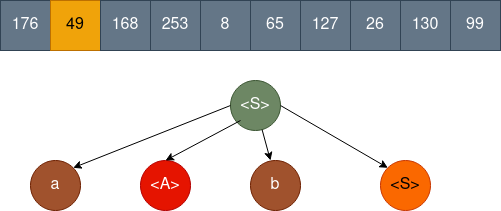
\includegraphics[scale=0.6]{parsing_tree_02.png}
	\caption{Genotype-phenotype mapping, step 2}
\end{figure}

\clearpage

Our current string is $a\:a\:b\:{<}C{>}\:b\:{<}S{>}$, the index value is $i = 2$, and the codon value is $168$. The leftmost nonterminal symbol is ${<}C{>}$, which has $3$ productions defined. So we calculate $168\:\:MOD\:\:3\:=\:0$, and apply the production at index $0$, which is ${<}C{>}\:::=\:c\:{<}C{>}$.

\begin{figure}[H]
	\centering
	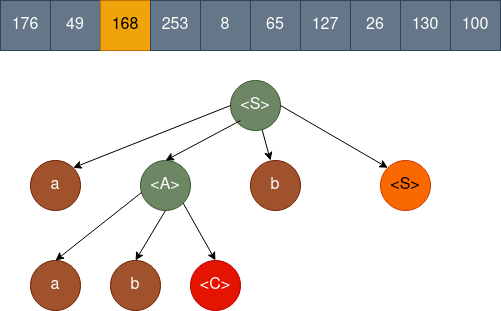
\includegraphics[scale=0.6]{parsing_tree_03.png}
	\caption{Genotype-phenotype mapping, step 3}
\end{figure}

Our current string is $a\:a\:b\:c\:{<}C{>}\:b\:{<}S{>}$, the index value is $i = 3$, and the codon value is $253$. The leftmost nonterminal symbol is ${<}C{>}$, which has $3$ productions defined. So we calculate $253\:\:MOD\:\:3\:=\:1$, and apply the production at index $1$, which is ${<}C{>}\:::=\:{<}C{>}\:d\:{<}C{>}$.

\begin{figure}[H]
	\centering
	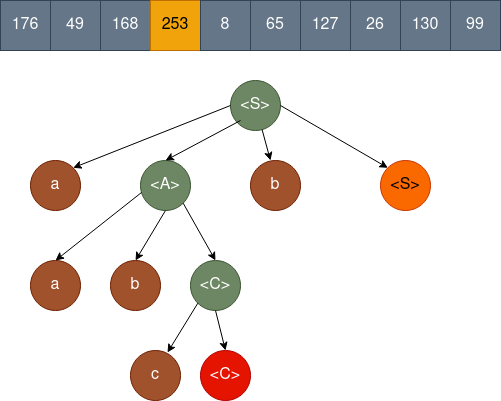
\includegraphics[scale=0.6]{parsing_tree_04.png}
	\caption{Genotype-phenotype mapping, step 4}
\end{figure}

Our current string is $a\:a\:b\:c\:{<}C{>}\:d\:{<}C{>}\:b\:{<}S{>}$, the index value is $i = 4$, and the codon value is $8$. The leftmost nonterminal symbol is ${<}C{>}$, which has $3$ productions defined. So we calculate $8\:\:MOD\:\:3\:=\:2$, and apply the production at index $2$, which is ${<}C{>}\:::=\:a$.

\begin{figure}[H]
	\centering
	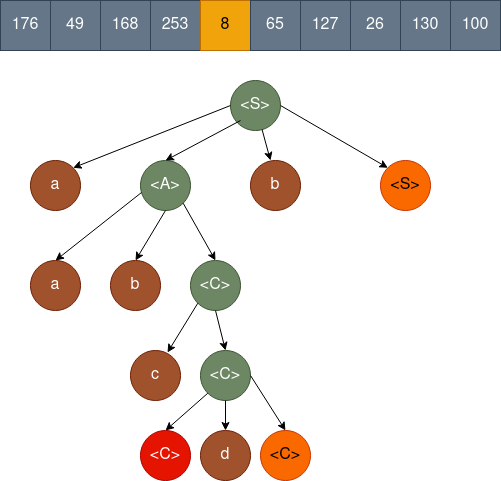
\includegraphics[scale=0.6]{parsing_tree_05.png}
	\caption{Genotype-phenotype mapping, step 5}
\end{figure}

\clearpage

Our current string is $a\:a\:b\:c\:a\:d\:{<}C{>}\:b\:{<}S{>}$, the index value is $i = 5$, and the codon value is $65$. The leftmost nonterminal symbol is ${<}C{>}$, which has $3$ productions defined. So we calculate $65\:\:MOD\:\:3\:=\:2$, and apply the production at index $2$, which is ${<}C{>}\:::=\:a$.

\begin{figure}[H]
	\centering
	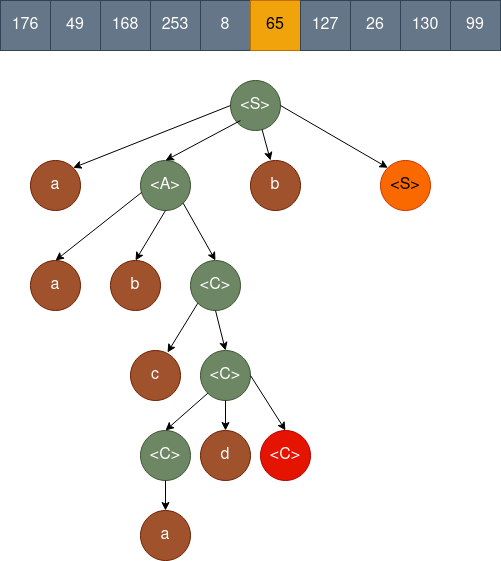
\includegraphics[scale=0.6]{parsing_tree_06.png}
	\caption{Genotype-phenotype mapping, step 6}
\end{figure}

\clearpage

Our current string is $a\:a\:b\:c\:a\:d\:a\:b\:{<}S{>}$, the index value is $i = 6$, and the codon value is $127$. The leftmost nonterminal symbol is ${<}S{>}$, which has $2$ productions defined. So we calculate $127\:\:MOD\:\:2\:=\:1$, and apply the production at index $1$, which is ${<}S{>}\:::=\:{<}C{>}\:d\:{<}A{>}$.

\begin{figure}[H]
	\centering
	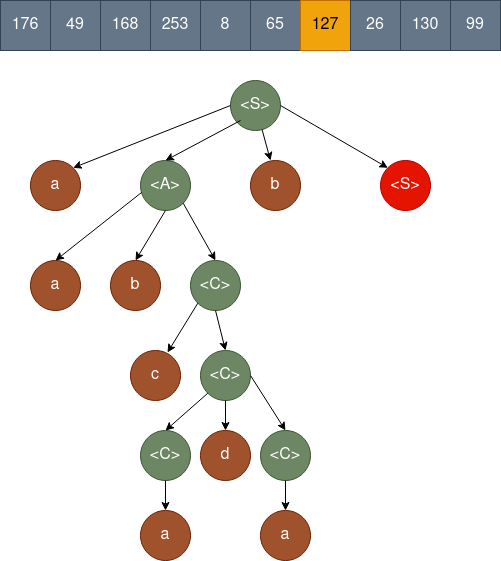
\includegraphics[scale=0.6]{parsing_tree_07.png}
	\caption{Genotype-phenotype mapping, step 7}
\end{figure}

\clearpage

Our current string is $a\:a\:b\:c\:a\:d\:a\:b\:{<}C{>}\:d\:{<}A{>}$, the index value is $i = 7$, and the codon value is $26$. The leftmost nonterminal symbol is ${<}C{>}$, which has $3$ productions defined. So we calculate $26\:\:MOD\:\:3\:=\:2$, and apply the production at index $2$, which is ${<}C{>}\:::=\:a$.

\begin{figure}[H]
	\centering
	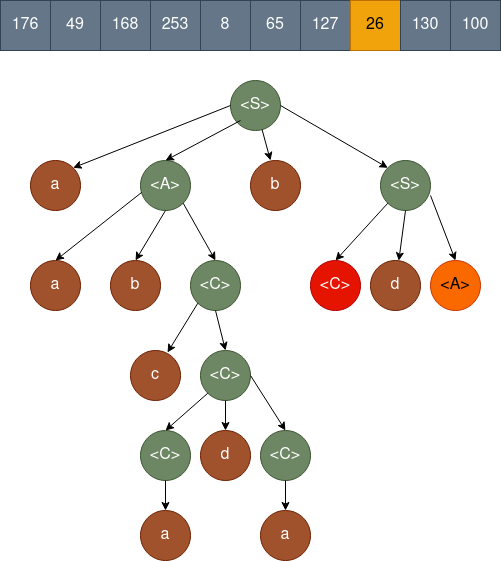
\includegraphics[scale=0.6]{parsing_tree_08.png}
	\caption{Genotype-phenotype mapping, step 8}
\end{figure}

\clearpage

Our current string is $a\:a\:b\:c\:a\:d\:a\:b\:a\:d\:{<}A{>}$, the index value is $i = 8$, and the codon value is $130$. The leftmost nonterminal symbol is ${<}A{>}$, which has $3$ productions defined. So we calculate $130\:\:MOD\:\:3\:=\:1$, and apply the production at index $1$, which is ${<}A{>}\:::=\:a\:b\:{<}C{>}$.

\begin{figure}[H]
	\centering
	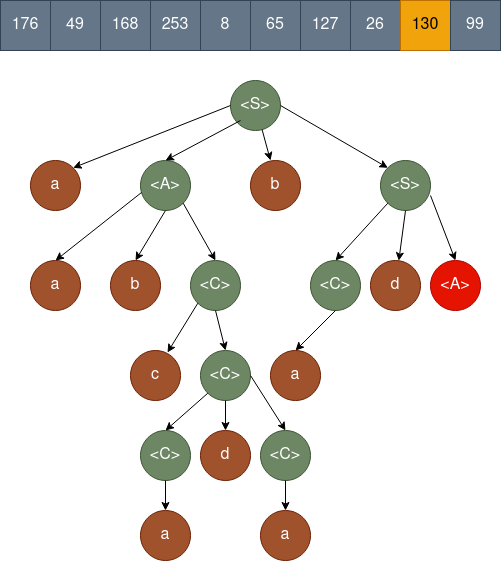
\includegraphics[scale=0.6]{parsing_tree_09.png}
	\caption{Genotype-phenotype mapping, step 9}
\end{figure}

\clearpage

Our current string is $a\:a\:b\:c\:a\:d\:a\:b\:a\:d\:a\:b\:{<}C{>}$, the index value is $i = 9$, and the codon value is $100$. The leftmost nonterminal symbol is ${<}C{>}$, which has $3$ productions defined. So we calculate $100\:\:MOD\:\:3\:=\:1$, and apply the production at index $1$, which is ${<}C{>}\:::=\:c\:{<}C{>}$.

\begin{figure}[H]
	\centering
	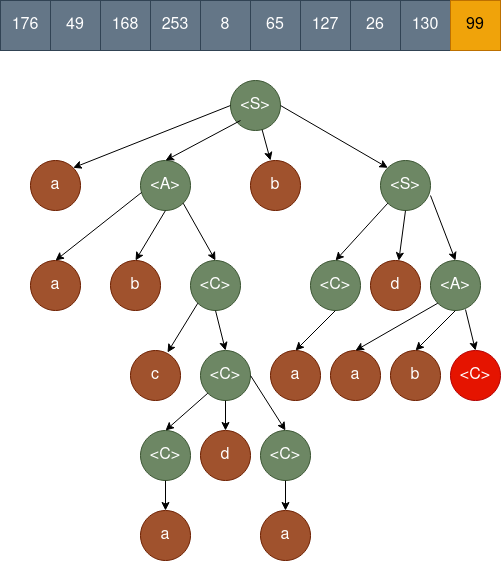
\includegraphics[scale=0.6]{parsing_tree_10.png}
	\caption{Genotype-phenotype mapping, step 10}
\end{figure}

\clearpage

Our current string is $a\:a\:b\:c\:a\:d\:a\:b\:a\:d\:a\:b\:c\:{<}C{>}$, the index value is $i = 10$. Since our codon array has only 10 elements, index $i = 10$ is out of bounds, but the mapping process is incomplete, so we apply the wrapping operator and set $i = 0$. The codon value is $176$. The leftmost nonterminal symbol is ${<}C{>}$, which has $3$ productions defined. So we calculate $176\:\:MOD\:\:3\:=\:2$, and apply the production at index $2$, which is ${<}C{>}\:::=\:a$.

\begin{figure}[H]
	\centering
	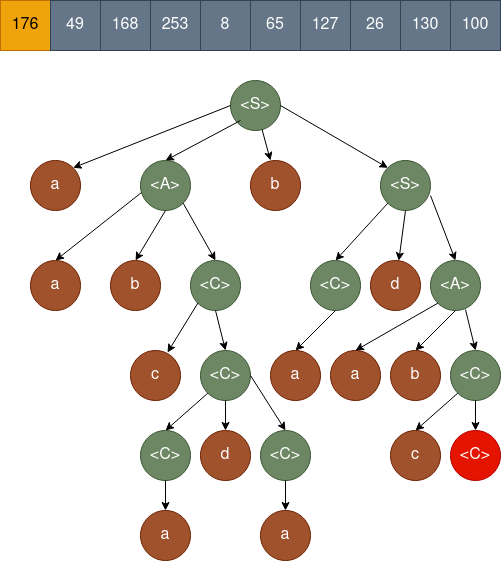
\includegraphics[scale=0.6]{parsing_tree_11.png}
	\caption{Genotype-phenotype mapping, step 11}
\end{figure}

\clearpage

Our current string is $a\:a\:b\:c\:a\:d\:a\:b\:a\:d\:a\:b\:c\:a$. Since there are no more nonterminal symbols in this string, the mapping process is finished, and this string is the final result of the mapping.

\begin{figure}[H]
	\centering
	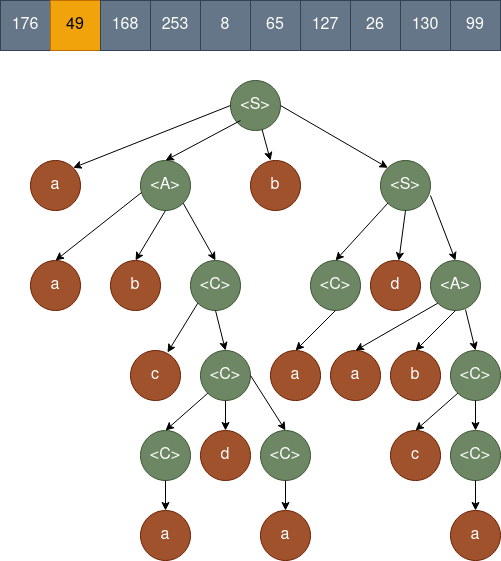
\includegraphics[scale=0.6]{parsing_tree_12.png}
	\caption{Genotype-phenotype mapping, step 12}
\end{figure}